%\documentclass[notes,10pt,aspectratio=169]{beamer}

%\documentclass[notes, 10pt,aspectratio=169]{beamer}
\documentclass[10pt,aspectratio=169]{beamer}


% Add this line to your preamble
%\setbeameroption{show notes on second screen=right}

%\usetheme{Singapore} %Boadilla, Madrid, default, etc. 
\usetheme[progressbar=frametitle]{metropolis}
\usecolortheme{rose} %beaver, dolphin, crane, 


%\setbeamersize{text margin left=4mm, text margin right=4mm}


\usecolortheme{default}

\usepackage[utf8]{inputenc}
\usepackage[T1]{fontenc}
\usepackage{lmodern}
\usepackage{xcolor}
\usepackage{tikz}
\usepackage{booktabs} % Required for \toprule, \midrule, \bottomrule
\usetikzlibrary{shapes.geometric, arrows, positioning}

\tikzstyle{block} = [rectangle, draw, text width=4cm, align=center, rounded corners, minimum height=1cm]
\tikzstyle{decision} = [rectangle, draw, text width=5cm, align=center, fill=blue!10, rounded corners, minimum height=1cm]
\tikzstyle{terminal} = [rectangle, draw, text width=4.5cm, align=center, fill=yellow!30, rounded corners, minimum height=1cm]
\tikzstyle{end} = [rectangle, draw, text width=5cm, align=center, fill=green!30, rounded corners, minimum height=1cm]
\tikzstyle{arrow} = [->, thick]



\usepackage{adjustbox}
%2. change the bullets 
\setbeamertemplate{itemize item}[triangle] %circle, square,... 


% 1. Define custom colors and set colors 
%\definecolor{myblue}{HTML}{003366}
\definecolor{accent}{RGB}{78,205,196}

%\setbeamercolor{title}{fg=white,bg=myblue}
\setbeamercolor{frametitle}{fg=black,bg=white}
%\setbeamercolor{normal text}{fg=mygray}
\setbeamercolor{block title}{fg=black,bg=blue}
%\setbeamercolor{block body}{fg=black,bg=white}

\setbeamercolor{item}{fg= orange!80} % Change bullet color
\setbeamercolor{button}{bg=orange, fg=white}





% 3. BibLaTeX settings
\usepackage[
  backend=biber,
  style=apa,
  citestyle=authoryear
]{biblatex}
\addbibresource{references.bib}

\title{Meetin with SPoints to discuss with Steve}
%\subtitle{A Mini Literature Overview}

\author{%
 Lucas Condeza
\inst{1} \and
   %\and
%  Coauthor Three\inst{3}
}
\institute{
  \inst{1} Yale University \\
}

\date{\today}

\begin{document}

%\begin{frame}
%  \titlepage
%\end{frame}





\begin{frame}{This meeting}
\begin{itemize}
        \item Learning evidence 
        \item Model of learning 
        \item Discrimination
            
\end{itemize}
\end{frame}
 


\begin{frame}{Learning}
\begin{itemize}
        \item Firms increase their offers more the higher the initial offers of the competitors. 
        
        
        \item The probability of making an external offer is decreasing on the value of the initial offers of the competitors. 
        
        \item There is bunching around the maximum initial offer. Firms might try to be the highest offer.  
\end{itemize}
\end{frame}
 



\begin{frame}%{Learning}
{
\def\sym#1{\ifmmode^{#1}\else\(^{#1}\)\fi}
\begin{tabular}{l*{7}{c}}
\hline\hline
                    &\multicolumn{1}{c}{(1)}&\multicolumn{1}{c}{(2)}&\multicolumn{1}{c}{(3)}&\multicolumn{1}{c}{(4)}&\multicolumn{1}{c}{(5)}&\multicolumn{1}{c}{(6)}&\multicolumn{1}{c}{(7)}\\
                    &\multicolumn{1}{c}{Increase}&\multicolumn{1}{c}{Increase}&\multicolumn{1}{c}{Increase}&\multicolumn{1}{c}{Increase}&\multicolumn{1}{c}{Increase}&\multicolumn{1}{c}{Increase}&\multicolumn{1}{c}{Has External Offer}\\
\hline
main                &                     &                     &                     &                     &                     &                     &                     \\
Avg. Gap            &       0.316\sym{***}&       0.155\sym{***}&       0.155\sym{***}&       0.139\sym{***}&       0.147\sym{***}&       0.071\sym{***}&                     \\
                    &     (0.006)         &     (0.010)         &     (0.010)         &     (0.016)         &     (0.019)         &     (0.020)         &                     \\
[1em]
Max. Gap            &                     &       0.110\sym{***}&       0.110\sym{***}&                     &      -0.021         &      -0.006         &                     \\
                    &                     &     (0.009)         &     (0.009)         &                     &     (0.029)         &     (0.028)         &                     \\
[1em]
gap\_from\_avg        &                     &                     &                     &                     &                     &                     &      -0.191\sym{***}\\
                    &                     &                     &                     &                     &                     &                     &     (0.032)         \\
[1em]
Constant            &       1.893\sym{***}&       1.375\sym{***}&       1.375\sym{***}&       1.381\sym{***}&       1.387\sym{***}&       1.511\sym{***}&      -2.012\sym{***}\\
                    &     (0.010)         &     (0.082)         &     (0.082)         &     (0.045)         &     (0.046)         &     (0.121)         &     (0.028)         \\
\hline
Observations        &       14133         &       14133         &       14133         &        2046         &        2046         &        2046         &       16164         \\
\hline\hline
\multicolumn{8}{l}{\footnotesize Average: is the difference between the mean of other firms' initial offers and own initial offer}\\
\multicolumn{8}{l}{\footnotesize Max Gap: is the difference between the highest other firm's initial offer and own initial offer.}\\
\multicolumn{8}{l}{\footnotesize Cols (1)-(3) use the population of initial offers that are not the highest, (4)-(6) only use the highest offer}\\
\multicolumn{8}{l}{\footnotesize Cols (4) and (6) include firm fixed effects}\\
\end{tabular}
}

\end{frame}

\begin{frame}{Learning(1)}
  \begin{figure}[H]
\caption{}
\label{fig:ie7_3}
\centering{}%
\begin{tabular}{cc}
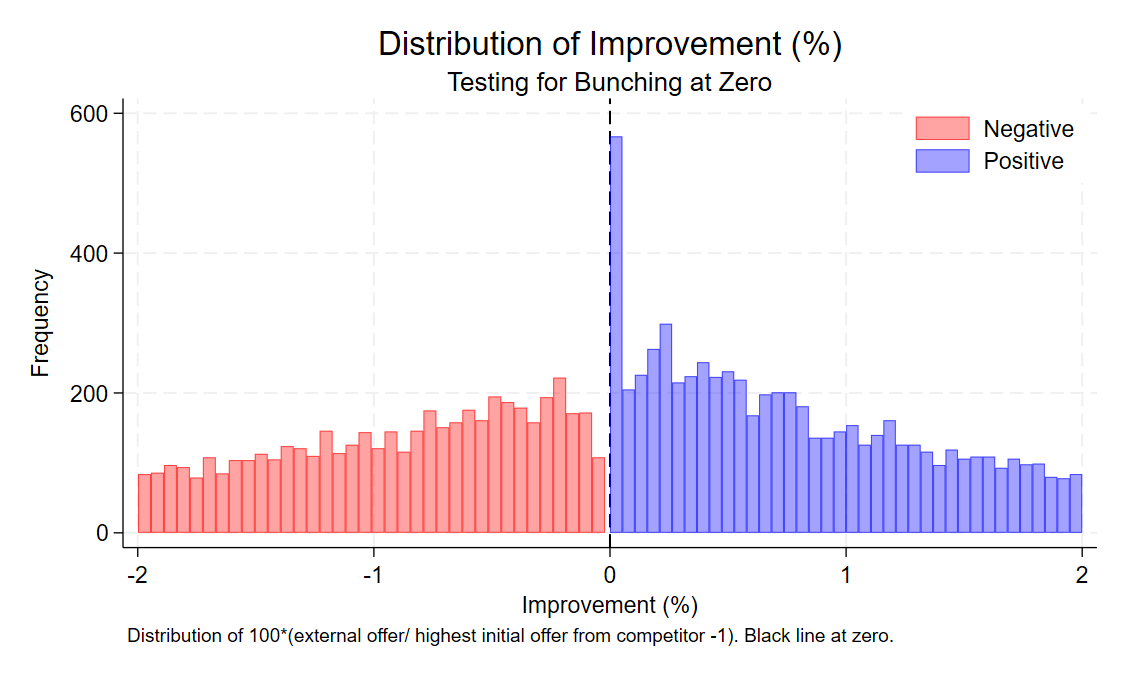
\includegraphics[scale=0.39]{../figures/IE7/IE7_hist_bunching_max(2).png} 
\end{tabular}
\end{figure}
\end{frame}

\begin{frame}{Other}

    \begin{itemize}
        \item For model of learning see the printout of model 5 
        \item How to determine whether there is some selection into the second stage? 
    \end{itemize}
    
\end{frame}


 
\end{document}